\documentclass[12pt]{article}
\usepackage{MinionPro}
\usepackage{CJK}
%\usepackage[scaled=0.85]{beramono}  %%% scaled=0.775
\usepackage[T1]{fontenc}
\usepackage{graphicx,booktabs,tabularx,psfrag}
\usepackage{xcolor}
\usepackage[a4paper]{geometry}
\usepackage{url}

\usepackage{pstool}

\usepackage{graphicx}
\begin{document}
\begin{CJK}{UTF8}{cwmb}
\renewcommand{\figurename}{圖}

\voffset=-1cm
\textwidth=5.6in
\textheight=9.2in

\newenvironment{num}
 {\leftmargini=6mm\leftmarginii=8mm
  \begin{enumerate}\itemsep=-2pt}
 {\end{enumerate}}

\newenvironment{sol}
 {\begin{quote}\mbox{}\llap{\color{blue}{解答:}\rule{10mm}{0pt}}\hspace*{-4pt}}{\end{quote}}


\thispagestyle{empty}
\fontsize{12}{20pt}\selectfont
\begin{center}
{\large\CJKfamily{cwyb}{經濟學原理下, 習題5}}\\[3mm]
劉彥佑 (R99628130)\\
李卿澄 (B97501046)\\
黃博億 (B99101014)\\
王祉婷 (B00704056)
\end{center}

\begin{num}
\item 
	\begin{num}
		\item $R^k=\frac{30+80-100}{100}=10\%$。
		\item $r^k=\frac{1+R^k}{1+\pi}-1=\frac{1+0.1}{1+0.03}-1=6.796\%$
		\item $10\%=R^k > R=6\%$,執行此投資比把錢放著生利息還好,當然應該投資之。
	\end{num}
\item 
	\begin{num}
		\item 甲欲貸入4,乙欲貸入1。
		\item 第1期期末之實質債券餘額:
\begin{figure}[htp]
\centering
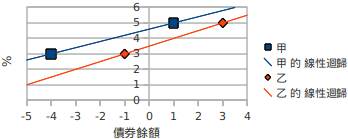
\includegraphics[scale=0.6]{2b.png}
\end{figure}
		\item 可貸資金市場之供需圖:
\begin{figure}[htp]
\centering
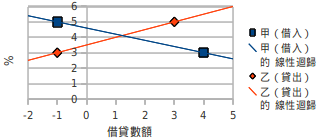
\includegraphics[scale=0.6]{2c.png}
\end{figure}
		\item 總合儲蓄與總合固定投資圖:
\begin{figure}[htp]
\centering
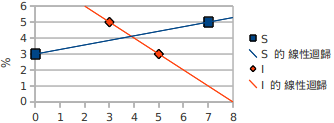
\includegraphics[scale=0.6]{2d.png}
\end{figure}
		\item 介於兩者之間。(依供需線為直線之假設,可解出利率為$\frac{37}{9}$)
		\item 大於0,因存在固定投資(參考(d),總合儲蓄於平衡時等於總合固定投資)。
		\item 低於39。利率越高總產出越高。利率為5\%時總產出為39,平衡時利率小於5\%,故其總產出不會超過39。
		\item 低於35。利率越低總消費越高。利率為3\%時總消費為35,平衡時利率大於3\%,故其總消費不會超過35。
		\item 總產出會高於總消費。總合儲蓄大於零,而總合儲蓄就是總產出減去總消費,故得知總產出大於總消費。
	\end{num}
\item 在國民所得均衡時,總合儲蓄會等於總合固定投資。商品總和需求$Y^d=C^d+I^d+G^d+(X-M)^d=Y^s$=GDP,總合儲蓄=$I^d$=3,104,590百萬元。
\item 仍然成立。借貸市場達成均衡代表企業借入了100億元,企業若不進行固定投資,其借入的需求是其支出減去收入,即其負儲蓄。由此可知,企業將借來的60億進行固定投資,而剩下的40億即是其負儲蓄,與課本之例子相較,總合儲蓄加上了企業的負儲蓄,短少40億元,總合固定投資也減少40億元,而總合儲蓄仍然等於總合固定投資。
\item
	\begin{num}
		\item $s_2=(\frac{b_2}{p_2}-\frac{b_1}{p_1})+i_2=-342.75+355.00=12.25$萬元,債券餘額為$\frac{b_1}{p_1}+12.25=-342.75$萬元。
		\item 以試算表軟體計算,至第19期期末時,債券餘額為-10.378298
萬元,至第20期即可還清貸款,由借入轉為貸出。
	\end{num}
\end{num}

\end{CJK}
\end{document}
